\documentclass[12pt,a4paper]{report}
\usepackage{tikz}
\usepackage{geometry}
\usepackage{amsmath}
\usepackage{graphicx}
\usepackage{listings}
\usepackage{xcolor}

\geometry{margin=1in}

% Define code style
\lstset{
  basicstyle=\ttfamily\footnotesize,
  keywordstyle=\color{blue},
  stringstyle=\color{red},
  commentstyle=\color{green!50!black},
  breaklines=true,
  frame=single,
  keepspaces=true,
  columns=fullflexible,
  showstringspaces=false
}

\begin{document}

% ---------------- COVER PAGE ----------------
\begin{titlepage}
    \centering
    \vspace*{1.8cm}
    {\LARGE \textbf{University of Chittagong}\par}
    {\Large Dept. of Computer Science \& Engineering\par}

    \vspace*{1.4cm}

    {\LARGE \textbf{DBMS Assignment}\par}
    \vspace{0.5cm}
    {\Large Tutorial-03\par}
    Course Title: Database Management Systems\par
    Course Code: CSE-414\par

    \vspace{1.2cm}
    \textbf{Submitted to}\par
    \vspace{0.3cm}
    Course Instructor\par
    Dr. Rudra Pratap Deb Nath\par
    Professor\par
    Dept. of Computer Science \& Engineering\par
    University of Chittagong\par

    \vspace{1.1cm}
    \textbf{Submitted by}\par
    \vspace{0.3cm}
    Team Name: ByteForge\par
    Name: Sheikh Tawsif Bin Aftab\par
    ID: 24701026\par
    Department: Computer Science and Engineering\par
    Semester: 4th Semester\par

    \vfill

    Submission Date:\par
    April 16, 2026
\end{titlepage}


% ---------------- ANSWER 1: CONCEPTUAL MODEL ----------------
\chapter*{Answer 1: Conceptual Model}
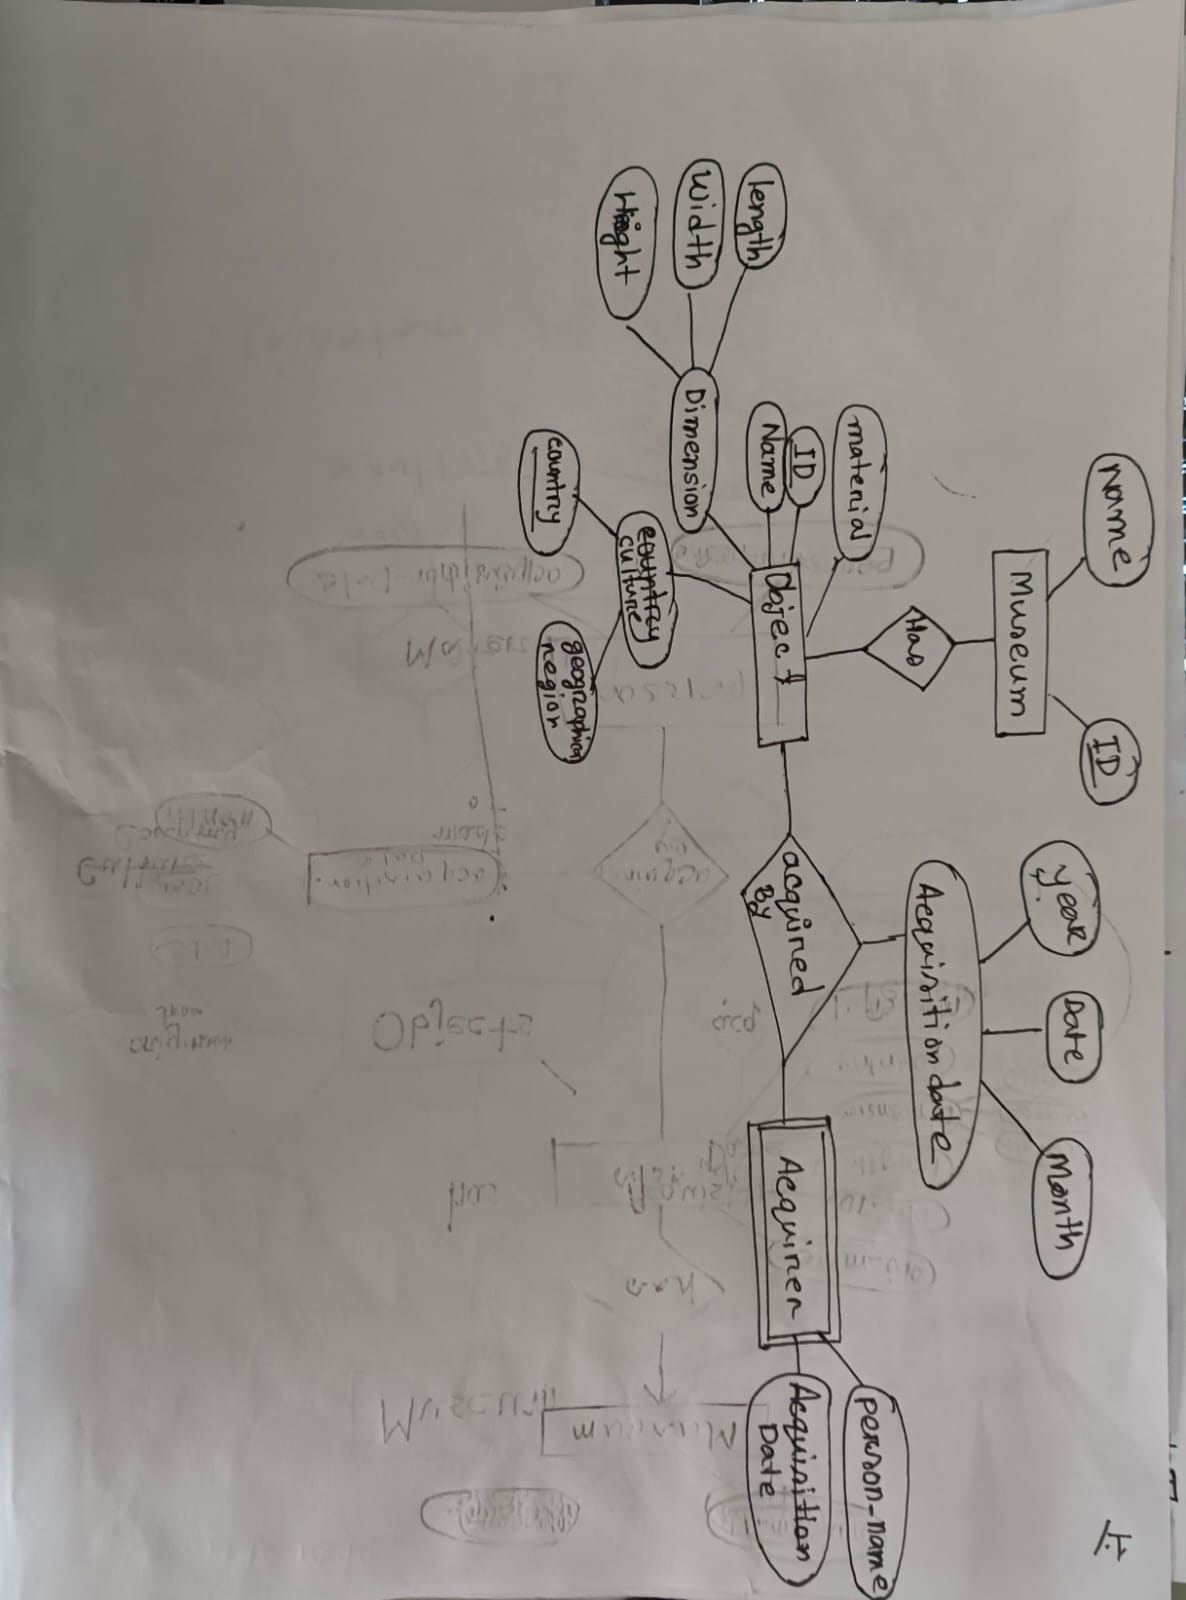
\includegraphics[width=0.95\textwidth]{Tutorial 3.jpeg}\par


% ---------------- ANSWER 2: DATA NOISE ANALYSIS ----------------
\chapter*{Answer 2: Data Noises}
\section*{Museum 1 Noises}
\begin{itemize}
  \item Inconsistent dimension formats: some rows only contain length and width, while others contain length, width, and height. Some records also use placeholders such as ``-'' instead of actual values.
  \item Mixed language values: several fields contain Dutch terms such as ``Aankoop'', ``Verwerving'', and ``19e eeuw'', which are not standardized with the rest of the dataset.
  \item Ambiguous descriptive fields: the values used for title, culture, and country-related information are not stored consistently in separate attributes.
  \item Missing measurements: several Museum 1 objects do not contain complete dimension values, which makes comparison and sorting difficult.
\end{itemize}

\section*{Museum 2 Noises}
\begin{itemize}
  \item Uncertain acquisition dates: values such as ``1877 (?)'' are not stored in a strict date format and introduce ambiguity.
  \item Missing transaction type: the transaction type column is empty for all Museum 2 rows.
  \item Redundant person fields: both ``Name'' and ``Names (all)'' appear in the source, which creates duplication and confusion about the primary acquirer name.
  \item Placeholder material values: strings such as \texttt{Stein <unbestimmt>} contain placeholder text and need cleaning before loading into the target model.
\end{itemize}


% ---------------- ANSWER 3: PYTHON SCRIPT ----------------
\chapter*{Answer 3: Python Script}
\lstinputlisting[language=Python]{../script.py}


% ---------------- ANSWER 4: SQL QUERIES ----------------
\chapter*{Answer 4: SQL Queries}
\begin{lstlisting}[language=SQL]
-- a)
SELECT Obj_Name, Obj_ID, Obj_Len, Obj_GeoRef
FROM museum
WHERE Obj_Len IS NOT NULL
ORDER BY Obj_Len DESC, Obj_ID ASC;

-- b)
SELECT Obj_Name, Obj_ID, Obj_Len
FROM museum
WHERE Obj_ID = 'IV Ca 4581';

-- c)
SELECT Mus_Name, COUNT(*) AS total_items
FROM museum
GROUP BY Mus_Name
ORDER BY total_items DESC, Mus_Name ASC
LIMIT 1;

-- d)
SELECT
    TRIM(SUBSTRING_INDEX(Obj_GeoRef, ';', 1)) AS Country_Origin,
    COUNT(*) AS total_objects
FROM museum
WHERE Obj_GeoRef IS NOT NULL
GROUP BY TRIM(SUBSTRING_INDEX(Obj_GeoRef, ';', 1))
ORDER BY total_objects DESC, Country_Origin ASC;

-- e)
SELECT Per_Name AS Acquirer, COUNT(*) AS total_items
FROM museum
WHERE Per_Name IS NOT NULL
GROUP BY Per_Name
ORDER BY total_items DESC, Acquirer ASC;

-- f)
SELECT Obj_Name, COUNT(*) AS total_count
FROM museum
WHERE Obj_Name IS NOT NULL
GROUP BY Obj_Name
ORDER BY total_count DESC, Obj_Name ASC;
\end{lstlisting}

\end{document}
